\begin{figure}
    \centering
    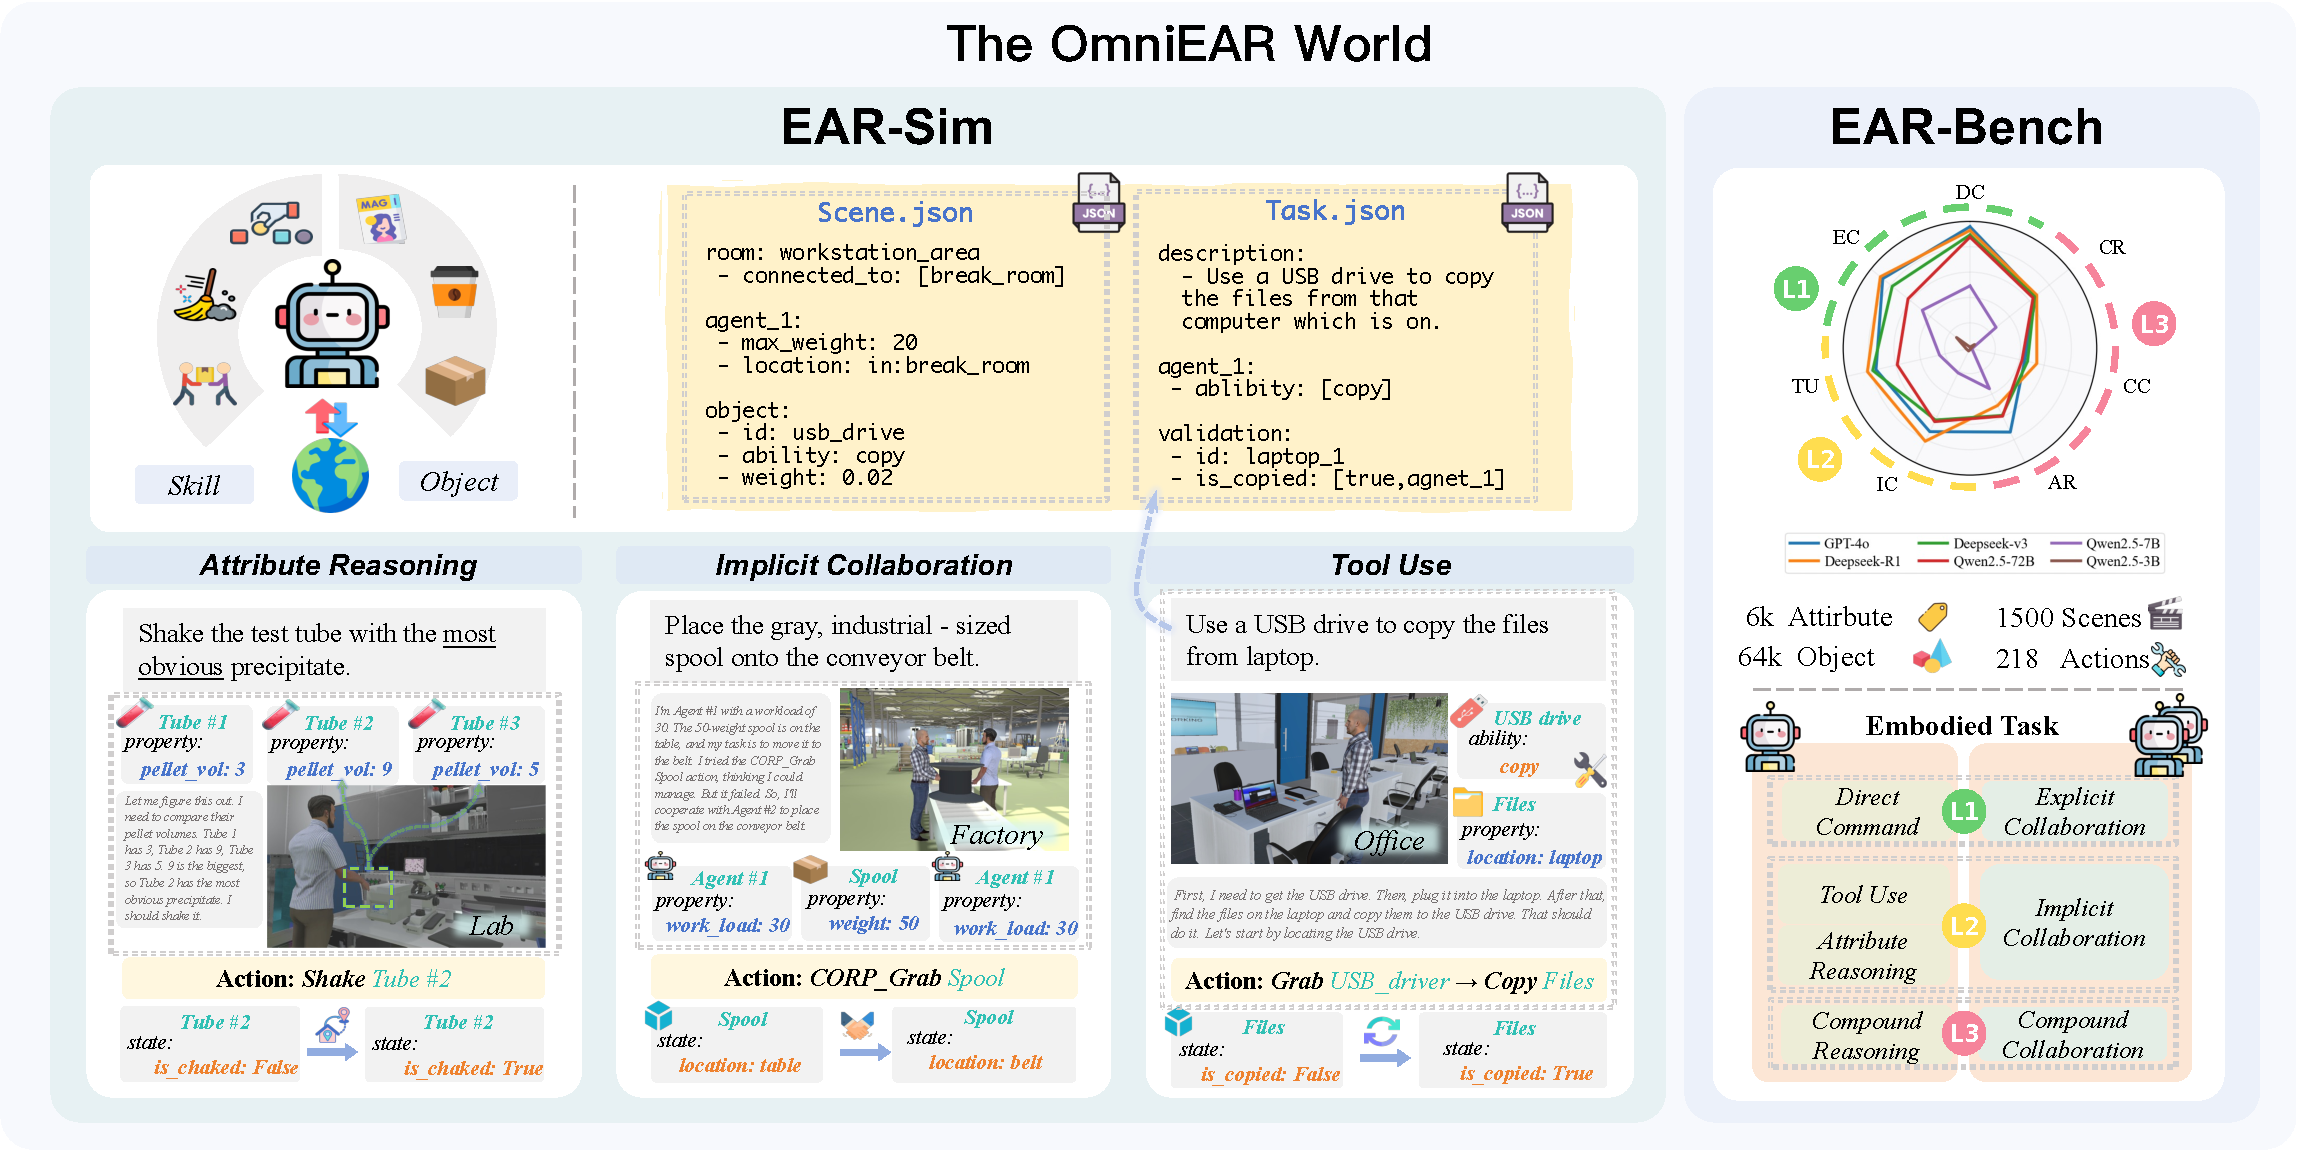
\includegraphics[width=1\linewidth]{figures/main.pdf}   \caption{Overview of the \framework framework comprising three integrated components: \textbf{\simulator} (left) uses structured text representation to model environments with objects, agents, and spatial relationships, enabling dynamic tool-capability binding and physics-constrained collaboration; \textbf{\benchmark} (right) presents our comprehensive evaluation matrix spanning single-agent and multi-agent tasks across increasing cognitive complexity levels.}
 
    \label{fig:main-overview}
\end{figure}
\section{Introduction}
Large language models have achieved remarkable success in complex reasoning tasks\citep{brown2020language,wei2022chain}, yet their ability to reason about embodied environments remains poorly understood. In embodied tasks, agents must understand how object properties affect what actions are possible, recognize when their capabilities are insufficient for a task, and determine when collaboration becomes necessary \citep{ahn2022icanisay, wu2023embodiedtaskplanninglarge}. These reasoning abilities fundamentally differ from abstract problem-solving, as they require understanding the physical principles that govern real-world interactions.

Current evaluation approaches fail to capture this embodied reasoning complexity. Existing benchmarks model environments through discrete states like open/closed doors or picked/placed objects \citep{shridhar2020alfredbenchmarkinterpretinggrounded, puig2018virtualhomesimulatinghouseholdactivities}, overlooking continuous properties such as weight, temperature, or material composition that determine action feasibility. Tool usage evaluations typically provide fixed action sets \citep{chang2024partnrbenchmarkplanningreasoning,huang2022inner}, missing how agents should reason about capability gaps. Multi-agent benchmarks rely on explicit collaboration instructions or efficiency metrics \citep{kang2025vikircoordinatingembodiedmultiagent, zhang2024buildingcooperativeembodiedagents}, rather than examining whether agents can recognize when tasks exceed individual abilities. This evaluation paradigm cannot assess understanding of embodied principles.

% The core challenge is that real-world embodied reasoning emerges from understanding environmental realities rather than following instructions.
The core challenge is that real-world embodied reasoning emerges from understanding environmental realities and task requirements. 
When objects are too heavy for single agents, collaboration naturally becomes necessary. When tasks require manipulating materials beyond native capabilities, tools provide the solution. When spatial layouts limit individual reach, coordinated action enables task completion \citep{zeng2022socraticmodelscomposingzeroshot, wang2023voyageropenendedembodiedagent}. Current benchmarks rely on static tool sets and explicit collaboration instructions, preventing assessment of how models reason about capability acquisition and coordination needs based on task requirements.

We introduce \framework, a comprehensive framework for evaluating agent reasoning in embodied tasks. Our key insight is that embodied reasoning requires understanding how physical properties shape possible actions, how capability limitations necessitate tools, and how task demands drive collaboration.
% By designing scenarios where successful strategies must emerge from this understanding rather than explicit guidance, we can assess whether models genuinely comprehend the principles governing embodied interactions.
By designing scenarios where agents must dynamically acquire capabilities and autonomously determine coordination strategies based on task requirements, we can assess whether models genuinely comprehend the principles governing embodied interactions.

\framework employs text-based environment representation to efficiently model rich physical properties while enabling large-scale evaluation. The framework comprises three integrated components: \simulator captures detailed object attributes and spatial relationships while supporting dynamic capability evolution through tool acquisition; an automated pipeline generates diverse scenarios where task solutions naturally depend on understanding embodied principles; and \benchmark provides systematic evaluation through 1,500 scenarios across household and industrial domains.

Our evaluation focuses on three core aspects of embodied reasoning. First, we assess how agents reason about object properties like weight, material, and temperature when determining feasible actions, requiring comparison and inference about continuous attributes. Second, we examine whether agents recognize when tasks demand capabilities beyond their current abilities and plan appropriate tool acquisition. Third, we evaluate autonomous coordination decisions, testing whether agents identify when task requirements exceed individual capacities without explicit collaboration instructions. These capabilities reflect fundamental aspects of embodied intelligence.

% Systematic evaluation reveals significant gaps in current models' embodied reasoning abilities. Leading models achieve 73-85\% success when given explicit guidance about tools or collaboration. However, performance drops sharply when agents must infer these needs from situational understanding: tool reasoning success falls to 38\%, coordination efficiency reaches only 40\% of optimal, and scenarios requiring integrated reasoning show 52\% failure rates. These results demonstrate that models struggle to derive appropriate strategies from understanding embodied principles.

Systematic evaluation reveals fundamental gaps in current models' embodied reasoning abilities. While achieving 85-96\% success on explicit instructions, performance degrades sharply when reasoning must emerge from physical constraints. Tool reasoning drops to 56-85\% when models must infer capability needs, and implicit collaboration falls to 63-85\% compared to 88-92\% with explicit coordination. Compound tasks show the steepest decline, with failure rates exceeding 50\%. Paradoxically, complete environmental information harms coordination performance, suggesting models cannot filter task-relevant from irrelevant constraints. Even reasoning-specialized models, which excel at logical planning, fail to ground physical constraints effectively, demonstrating that current architectures lack the mechanisms necessary for autonomous embodied decision-making.

Our analysis uncovers important patterns in model capabilities. Smaller models cannot maintain the planning state necessary for multi-step reasoning about tools and coordination. Reasoning models excel at logical planning but struggle to ground abstract concepts in concrete physical properties. While supervised fine-tuning improves single-agent performance, these gains fail to transfer to multi-agent scenarios, suggesting that coordination reasoning requires architectural capabilities beyond current training approaches.

In summary, our contributions are:

\begin{itemize}
\item We present \framework, a framework that evaluates embodied reasoning through scenarios requiring agents to understand how physical properties determine actions, capabilities, and coordination needs, addressing fundamental gaps in current evaluation methods.

\item We develop EAR-Bench, a benchmark of 1,500 scenarios with continuous physical properties and dynamic capabilities, supported by \simulator and an automated generation pipeline.

\item We provide empirical evidence that current language models lack core embodied reasoning capabilities, with performance degrading over 60\% when moving from explicit instructions to embodied reasoning, revealing critical requirements for advancing embodied AI.
\end{itemize}